\subsection{Myo armband}

To acquire EMG-signals the Myo armband (MYB) from Thalmic Labs is used. It contains eight dry stainless-steel electrode pairs placed inside the armband. The advantage of using dry electrodes is that they do not need to be disposed after use, in contrary to conventional gel electrodes. Thus, MYB can be reused for all subjects participating in the project, which provides less time consuming experiments. An additional usability advantage is that it communicates wirelessly to external devices via Bluetooth 4.0, leaving no loose wires to possibly limit mobility or distort connection. \\ 
MYB acquires EMG signals in an 8-bit resolution. Instead of acquiring the signal in millivolts, the output is scaled to decimal numbers between -1 and 1. However, the amplitude of the EMG signal output is still proportional to muscle contraction intensity. To avoid signal frequencies from the power grid to interfere with the EMG signal, an analogue notch filter at 50 Hz is built in the MYB. This is, however, the only analogue filter implemented in the MYB, and as it has a sample rate of 200 Hz, which is inside the EMG spectrum (10-500 Hz), the acquired EMG signal will likely be aliased. The implementation of a digital anti-aliasing filter would therefore be a trivial task and extracting features that represents the frequency content of the signal might not be useful. Additionally, MYB contains a 9 axes inertial measurement unit, but will not be utilized in this project and therefore not elaborated further. \\
During the initialization of using MYB the user has to follow two calibration steps: the warm up and the synchronization. In the warm-up step, MYB is establishing a strong electrical connection between the skin and the armband, which reduces skin-electrode impedance and enables the electrodes to transduce properly. This happens as the user's skin becomes more moist from light sweating, which works similar to the gel in conventional EMG electrodes. During the synchronization step the MYB determines its orientation in space, its position and on which arm it is placed, based on a wrist extension movement the user must perform. 
MYB works most optimally when tightly fit on the thickest part of the arm. To ensure a close fit, a set of clips can be used if necessary. 


\begin{figure}[H]                 
	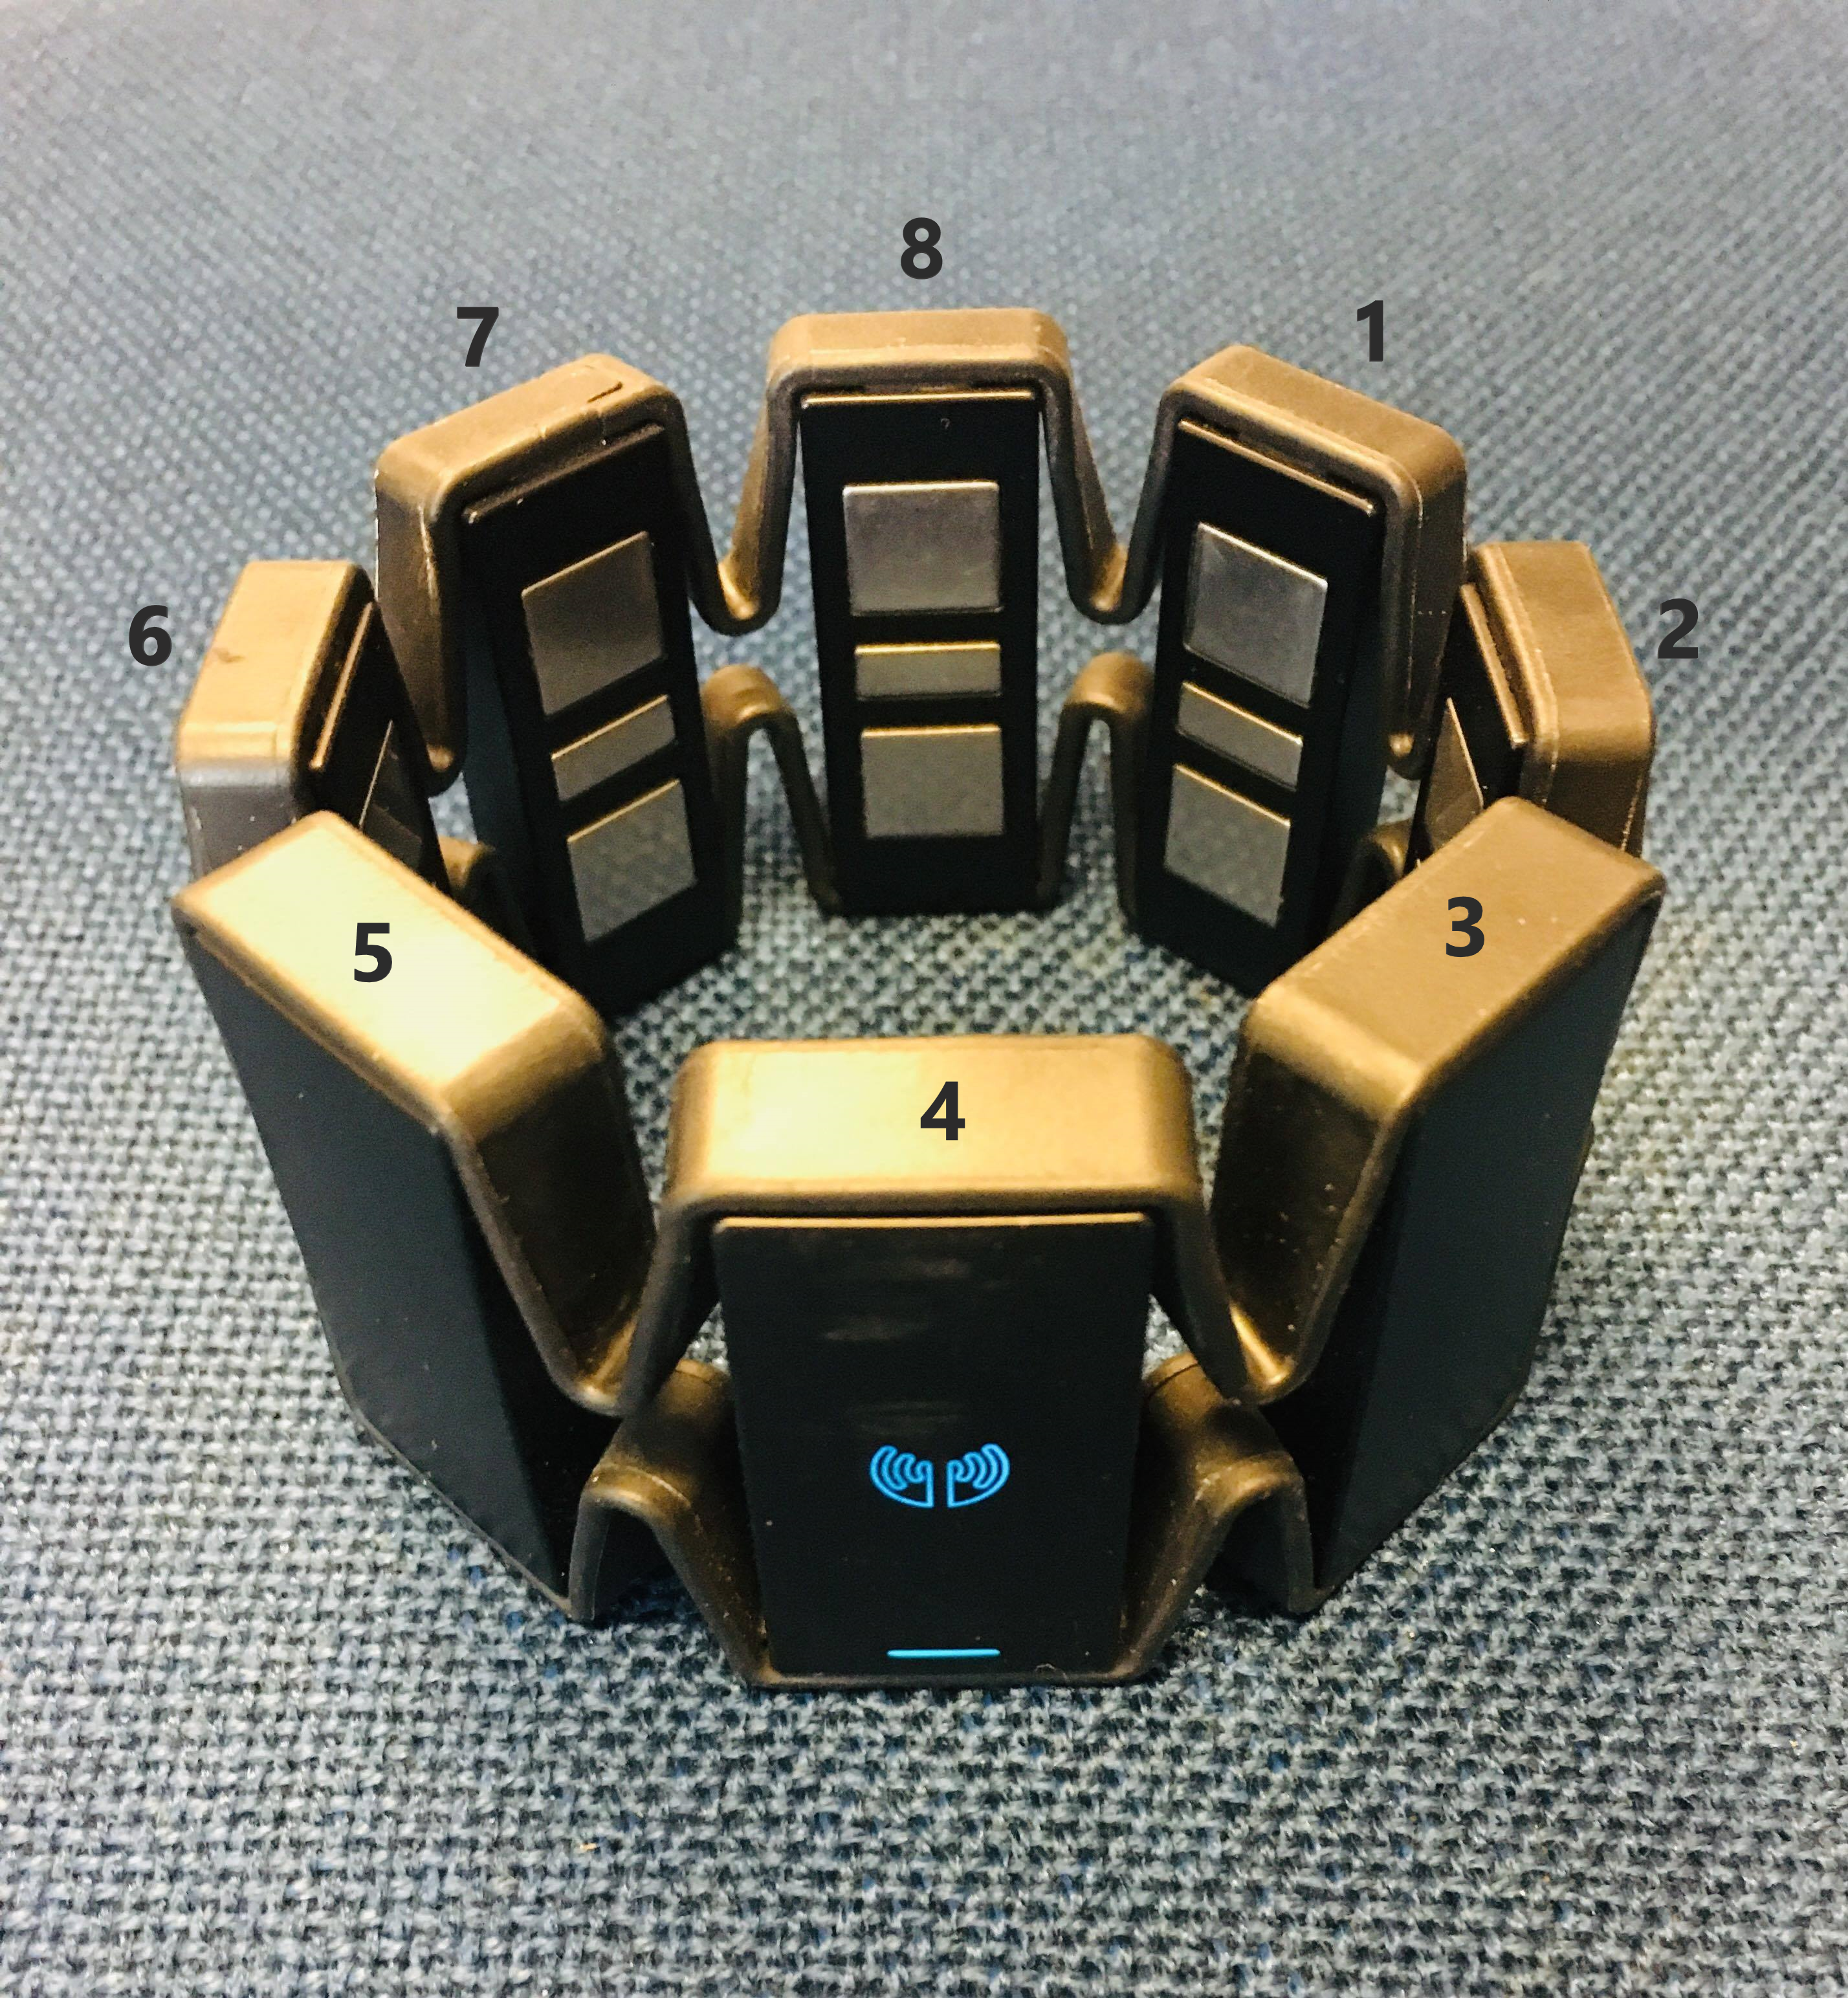
\includegraphics[width=.4\textwidth]{figures/MYB}  
	\caption{}
	\label{fig:MYB} 
\end{figure}